\documentclass[11pt,a4paper]{article}
\usepackage[top=2cm,left=2cm,right=2cm,footskip=0.75in]{geometry}
\usepackage{graphicx}
\usepackage{floatrow}
\usepackage{amsmath,amssymb}
\usepackage{url}
\usepackage[utf8x]{inputenc}
\usepackage{setspace}
\usepackage{multicol}
\usepackage{etoolbox}

\setstretch{1.1}
% \usepackage[document]{ragged2e}
\setcounter{section}{26}  % this is a section 27 of the proposal form

% \setlength{\oddsidemargin}{0.25in}
% \setlength{\textwidth}{6.5in}
% \setlength{\topmargin}{0in}
% \setlength{\textheight}{8.5in}

\newcommand{\myurl}[1]{\footnote{\url{#1}}}

\usepackage{caption}
\captionsetup[figure]{labelfont={bf},name={Fig.},labelsep=period}

\usepackage{fontspec}
\setmainfont{Calibri}

% \usepackage{fontspec}
% \setmainfont[Path=/System/Library/Fonts/,
%     BoldItalicFont=calibriz.ttf,
%     BoldFont      =calibrib.ttf,
%     ItalicFont    =calibrii.ttf]{calibri.ttf}

\renewcommand{\bold}{\textbf}
\graphicspath{ {./images/} }

\begin{document}

\title{\Large Computational Toolbox for Discovery of Prognostic Markers in Survival Analysis from Gene Expression Data: Description of the Research Project}
\author{}
\date{}
\maketitle
\vspace*{-1cm}

\bold{We propose a project to design and develop an interactive, visualization-based exploratory analysis toolbox to assist in finding molecular prognostic biomarkers from high-throughput molecular data and survival data obtained in clinical trials.} The project will devise computational and machine learning methods to search for biomarkers, encapsulate them within interactive components with graphical user interface, and provide visual programming to stitch these components into data analysis pipelines. The constructed methods and toolbox will support collaborations between the data scientists and domain experts – physicians, biomedical or pharma researchers – to sift through the molecular cell-response data of thousands of genes to find those that correlate most with the survival. The proposed tool will access existing models, ontologies, and knowledge bases to speed-up the interpretation and provide semi-automatic explanations of results. 


\bold{This is an applied project where we are teaming up with Genialis, a data science company specializing in computational support for precision medicine.} Genialis is currently in the process of registering with the FDA (US Food and Drug Administration) a first ever machine learning model that utilizes transcription data to predict cancer patients' response to treatment. To remain at the cutting edge of biomarker research, Genialis needs methods, tools, and visualizations to speed-up the discovery and improve communication of their data analysis results to their customers and regulatory agencies. On the other hand, the project will allow us, the proposing institution, to further advance our research into a combination of interactive visualizations and machine learning, and apply our new approaches to a challenging field of biomarker discovery.

\subsection{Scientific background, problem identification and objectives of the proposed research}

\subsubsection*{Scientific Background}

\bold{The project will contribute new methods and practical data exploration approaches to the field of survival analysis, and study how many covariates (genes with their expression) jointly affect survival.} Survival analysis is a set of statistical methods aimed at determining the life expectancy of the investigated population. Survival analysis studies the expected duration of time until an event, say, a cancer relapse after chemotherapy, or a recurrence of disease~\cite{pazdur2008endpoints}. Survival models, including the most famous one, the proportional hazards model, relate the time until the event to one or more covariates. In biomedicine, the covariates with a significant impact on survival are potential {\em markers}, a characteristic of a biological system we can objectively measure and use as an indicator of the system's state. For example, in cancer, markers may differentiate between patients that respond to treatment and those where the treatment has no effect.

\bold{Based on markers, we can predict the success of treatment and choose the right therapy for individual patient. Identification of good markers is thus essentials for advancements of medicine and treatment of diseases, and crucial to the development of personalized medicine.} Because improving survival is a direct benefit to the patient, it is very important to understand how participants respond to various forms of treatment. The treatment should thus be selected based on patient's state and characteristics, which are defined through a set of markers. Markers may be clinical, related to patient's symptoms, or biological, related to some measurements on molecular level, like concentration of specific protein or expression of particular gene or set of genes. Markers may refer to a single measurement of state, or to a group of measurements possibly related through a prognostic model or a network~\cite{Sonawane2019}.

\bold{High-throughput sequencing can be used to measure the degree of activity of genes in biological samples. In the recent years, attention has turned from simple single-gene DNA markers to complex multi-gene markers of gene expression.} The amount of mRNA in a biological sample that corresponds to a particular gene is correlated to gene's activity and is referred to as gene expression. High-throughput sequencing allows us to determine the expression of all genes in the organism, and hence provide a tool to assess the state of the biological system. A gene can be considered as a biomarker of survival if the survival function is substantially different in a subpopulation where gene is expressed compared to when it is not (see Fig.~\ref{fig:km-marker}). Note that this definition is vague, as it requires the threshold for gene expression, and quantification and a subsequent threshold for the difference between survival function. Moreover, sets of genes rather than single genes are typically used to capture diverse {\em biologies} in a sample, e.g. a tendency for blood vessel formation, or priming for immune response. A validated and effective gene expression-based biomarker discovery process can be an incredibly valuable and often a necessary tool in drug discovery, development, and diagnostic research~\cite{MonforteMcPhail2005}. It has shaped the discovery of biomarkers in disease such as cancer~\cite{HENRY2012140}, XXX.

\begin{figure}
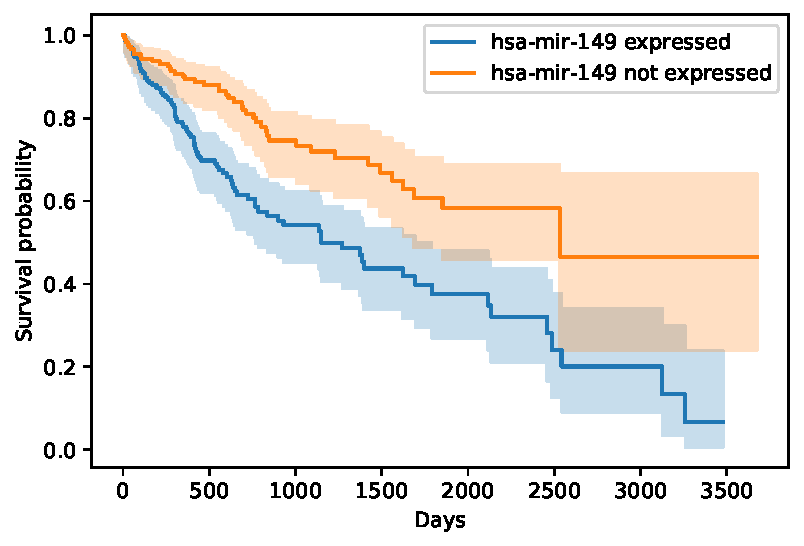
\includegraphics[width=0.48\textwidth]{hsa-mir-149}\hfill
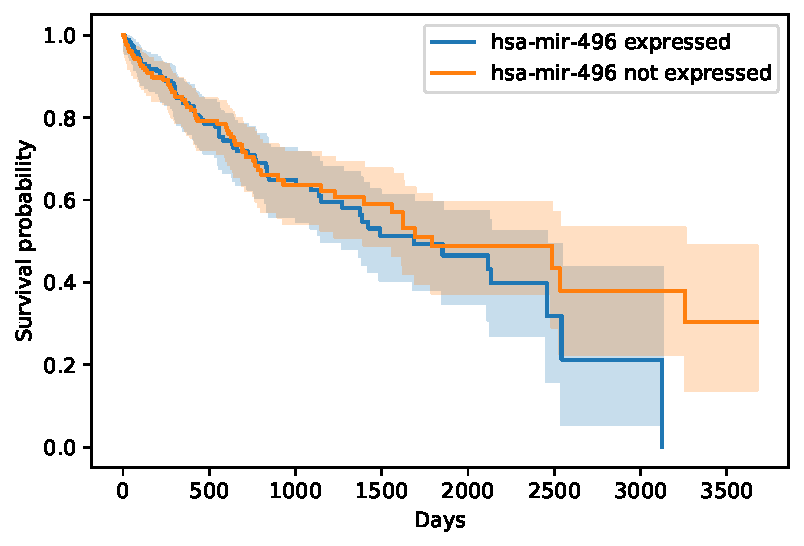
\includegraphics[width=0.48\textwidth]{hsa-mir-496}
\caption{\bold{An example of a Kaplan-Meier plot for two gene expression-dependent conditions associated with patient survival.} In panel a), the survival function is substantially higher for a group of patients with highly expressed microRNA hsa-mir-149. The difference is not so evident in the panel b) and microRNA hsa-mir-496. We could say that hsa-mir-149 is hence a better biomarker for survival. In biomarker discovery, one of the tasks is to rank genes and RNA molecules according to the degree of separation between corresponding survival signatures when a gene is expressed and not expressed.}
\label{fig:km-marker}
\end{figure}

\bold{Ideally, therefore, data-driven discovery of new biomarkers would only require survival data with corresponding gene expression profiles.} The discovery algorithms would then sift through all the genes and find those that best define groups with different survival function. But there are many difficulties and obstacles in this procedure, related to noisy data, small datasets in terms of the number of investigated samples, higher-order gene interactions, and inclusion of available additional knowledge. We examine these more closely next.

\subsubsection*{Problem Description}

\bold{There are three categories of problems and challenges we would like to address in the proposed project, affecting the computation methods to infer potential biomarkers, approaches to data fusion, and implementation:}
\begin{description}
	\item[Computational challenges, noise and overfitting.] The experimental data that addresses a specific survival problem, related to, say, impact of a new treatment or drug, is often expensive and hence small in sample size. A typical Phase 1 clinical trial often has less than 30 patients, and Phase 2 clinical trials with more than a hundred patients are an exception rather than the norm. Experimental noise related to sample collection and treatment, and to measurement of gene expression can be high. This setting can lead to false discoveries and overfitting. The problem is especially exposed when finding sets, or networks of genes that could serve as biomarkers, as the number of candidates (different sets of genes) grows exponentially with the desired size of the gene set. For instance, with $20.000$ protein coding genes, there are over $1,3$ trillion possible gene triples; even if we would computationally manage to examine them all, checking so many combinations will necessary lead to overfitting, where our results would apply well to the training data, but not generalize well to new cases. Besides noise and overfitting, computational challenges include those of finding gene expression thresholds (when is a gene expressed?) and aggregation functions (when is a set of genes collectively active?).
 	\item[Inclusion ob background knowledge.] Genes participate in molecular pathways, perform functions, and are associated to diseases and responses to chemicals and drugs. Knowledge about these and other gene annotations is stored in data bases such as GeneOntology~\cite{}, KEGG~\cite{}, PathwayCommons~\cite{}, CellMarker~\cite{}, and other. Examining gene sets as candidates for biomarkers could and should use these valuable sources of information, both for restricting the biomarker search space and interpreting the sets of best candidate genes (gene set enrichment). Such fusion of data and knowledge bases has generated some fascinating results in bioinformatics research~\cite{} but has been insufficiently explored in our target domain of survival biomarker discovery.
 	\item[Data exploration interface.] The past two decades have seen an emergence of a wide array of methods and statistical and machine learning tools to analyze high-throughput data from molecular biology. For survival analysis, however, there is no elegant toolbox with an intuitive user interface that would assist in biomarker discovery, support on-the-fly interactive exploratory data analysis, and offer easy construction of analytical pipelines. Available are excellent code libraries for survival analysis in R and Python, yet, for a systematic use, these are just building blocks that require advanced knowledge of programming to utilize and integrate. What we need instead are intuitive tools with flexible and exciting interactive interfaces to engage the end-users and data scientists in productive communication, data exploration and modeling.
\end{description}

\bold{In the project, we will address these three challenges through development of techniques and tools that will support interactive search for and exploration of potential biomarkers.} We aim to democratize the field of data-driven biomarker discovery by creating a versatile tool with interactive interface for intelligent analysis of survival data.

\subsubsection*{Project Aims}

\bold{The project will develop and apply a set of computational tools for inference of biomarkers from survival data.} We will integrate existing approaches to survival data-based biomarker scoring, survival modeling, and gene set enrichment analysis, and propose new techniques for survival-specific gene interactions, construction of biomarker candidate maps, and interpretation of constructed visualizations. We will devise means for heuristic search that will use published data bases on gene function and pathway annotation.

\bold{The project will empower domain experts and data miners use these tools in real-life applications - in real time and without the need to write computer code.} The project will embed computation methods into components with graphical user interfaces. We will enhance our own, open-source data mining platform Orange\myurl{http://orangedatamining.com}~\cite{Demsar2013,Curk2005,Godec2019} (Fig.~\ref{fig:orange-workflow}) with survival analysis capabilities. We will show that the resulting visual programming platform not only substantially reduces the complexity and user time spent on data analysis, but also enhances the collaboration and motivation of domain experts through informative visualizations and ability to steer the discovery process using domain knowledge. 

\bold{Finally, we would like to showcase the utility of the constructed toolbox.} In the application of project's approaches we will use a set of published and privately-owned (from participating SME) datasets of gene expression and corresponding clinical outcomes. The success of the project will be judged on use cases carried out by participating SME, and our ability to train them to independently use the results of the project.

\begin{figure}[htbp]
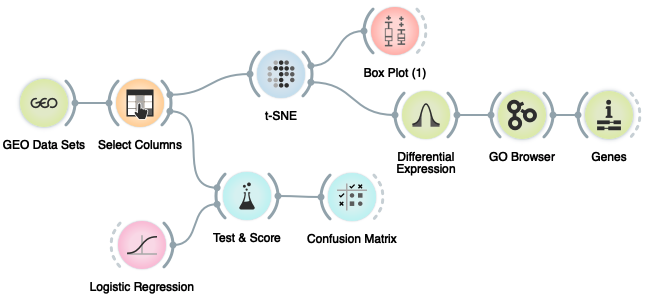
\includegraphics[width=0.7\textwidth]{orange-workflow}
\caption{\small\bold{A typical Orange bioinformatics workflow.} A figure shows an example where we have reanalyzed expression data from peripheral blood mononuclear cells (GDS5363), where the authors investigated if gene expression profiling could detect the onset of osteoarthritis~\cite{Ramos2014}. The workflow loads the data from Gene Expression Omnibus and defines the dependent variable (disease state, {\em Select Columns} widget). The upper branch checks the clustering structure of tissue samples ({\em t-SNE} widget), finds differentially expressed genes for selected samples, and analyzes their common characteristics through Gene Ontology term enrichment. In the lower branch, we check the investigators’ hypothesis directly and evaluate the accuracy of the predictions of a logistic regression model through cross-validation ({\em Test \& Score} widget). In the proposed project, we will develop similar-style workflows, but with components that will load, process, analyze and display survival data and discover biomarkers.}
\label{fig:orange-workflow}
\end{figure}

\begin{figure}[htbp]
\floatbox[{\capbeside\thisfloatsetup{capbesideposition={right,top},
capbesidewidth=0.4\textwidth}}]{figure}[\FBwidth]
{\caption{\small\bold{Most graphical components -- widgets in Orange are interactive.} We here show the content of several widgets from the workflow in Figure~\ref{fig:orange-workflow}. The user can, for instance, choose a subset of data points from the {\em t-SNE} visualization (data points with a yellow outline on the top right of the visualization), or data corresponding to a specific bar in the {\em Box Plot}, or a set of genes associated with a selected term from the {\em GO Browser}. In the {\em Differential Expression} widget, we can choose a set of differentially expressed genes in the tails of the gene score distribution plot. Most widgets contain both a control and a visualization part. The project will reuse some of the widgets from this visualization, include a t-SNE widget, and with design a set of specialized widgets for survival analysis and biomarker discovery which will similarly support interactivity.}
\label{fig:orange-interactivity}}
{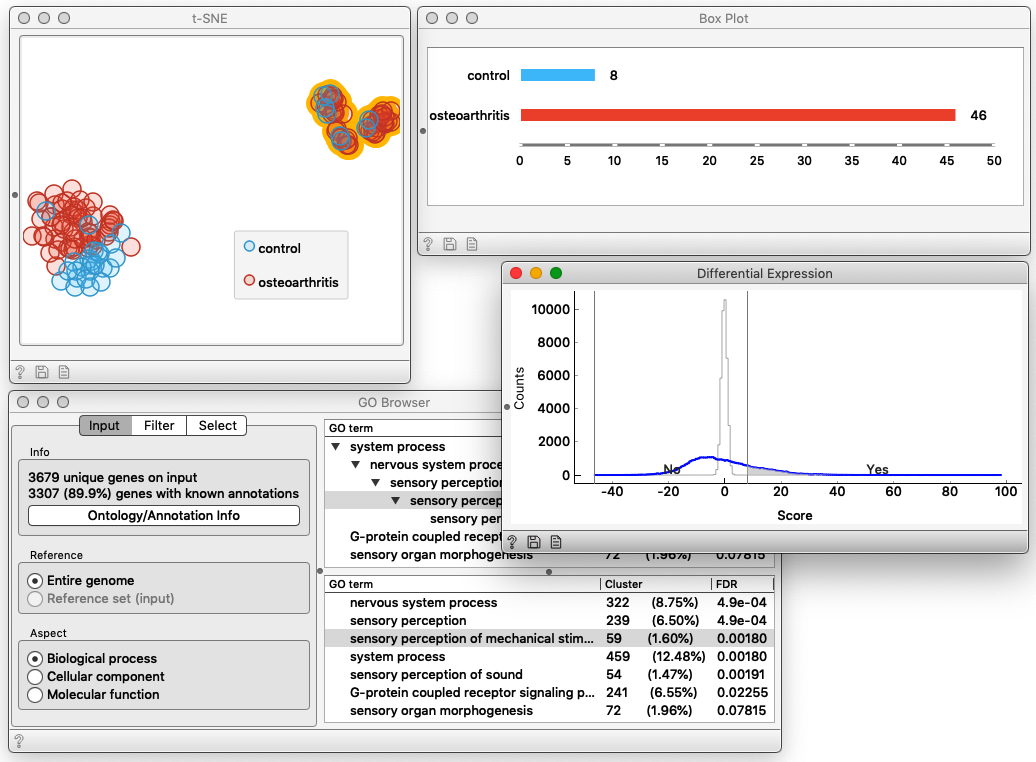
\includegraphics[width=0.6\textwidth]{orange-interactivity}}
\end{figure}

\subsubsection*{Anticipated Results}
The expected principal results of this project are:
\begin{enumerate}
	\item \bold{A bioinformatics library for biomarker discovery from survival data}. The library will be developed in Python and will be published in open-source on GitHub, together with documentation, unit-tests, and working examples;
	\item \bold{A biomarker discovery toolbox featuring visual programming interface, interactive visualizations, and interpretation and explanation of results}. The toolbox will support integration of external knowledge-bases, on-the-fly construction of analytical pipelines, interactive exploration of data and models (see Fig.~\ref{fig:orange-interactivity}), and domain knowledge-based guided data exploration;
	\item \bold{A set of use-cases developed in close collaboration with Genialis d.o.o.}, a participating SME. The use-cases will demonstrate the applicability of our software, showcase the power of toolbox's intuitive interface, and provide for instruction and educational material in dissemination of project's results.
\end{enumerate}

% \subsubsection*{Our Preliminary Results and Studies}

% gene network discovery, gene interactions, intelligent data visualization, embedding, Orange.

\subsection{State-of-the-art in the proposed field of research and survey of the relevant literature}

The log-rank test and Cox's proportional hazards model are most commonly used in the literature to compare survival between two different groups of observers~\cite{singh2011survival}. These two methods can be regarded as a baseline to design strategies for detecting predictive marker genes. In a nutshell, the search for marker genes, can be broken down into two subproblems: the grouping, or better, binarization of response variables (e.g., expression of the genes) and the search for promising predictive gene groups.

In clinical studies, biological markers are usually continuous variables obtained by various measurements. Establishing a cut-off point that represents the boundary between high and low gene expression, or more generally that distinguishes between high and low risk groups, may be essential for their use in clinical decision making~\cite{mazumdar2000categorizing}. Budczies et al.~\cite{budczies2012cutoff} propose several  approaches to selecting cut-off values: according to the distribution of the biological marker, by optimizing the interdependence of the target variable, such as response to treatment, or by finding a minimum p-value. The latter is the most common and selects the cut-off value according to the optimal difference in the survival outcome prediction between the groups~\cite{woo2020determination}. In general, however, finding the optimal value is a difficult problem that also depends on the study or research itself. Properly used procedures in finding the limit value are very important, as we may overestimate the true effect of the biological marker~\cite{Altman1991}.

Witten et al.\cite{witten2010survival} highlight the problem of finding predictive features in high-dimensional data. When the number of variables is many times greater than the number of cases, the usual statistical approaches to survival analysis are no longer sufficient. There are many different approaches to finding marker genes in published works. The set of possible candidates is narrowed by retaining in the first step only statistically significant differentially expressed genes, that is, genes that distinguish well between selected groups of observers, and in the second step further narrowing the set of possible candidates based on their individual statistical significance in survival analysis~\cite{wang2017identification,liao2018identification,zhang2011discovery,kim2013identification}. Relator et al.~\cite{relator2018identifying} are critical of such approaches because in this way we leave many possible combinations of genes untested. They suggest a solution that can detect the interactions of potential markers that would otherwise be omitted by conventional approaches. One of the important shortcomings of such an approach, as they themselves acknowledge, is computational complexity. To complete the test in a few days, they suggest splitting the data into smaller samples. They run the proposed solution over the individual samples and then combine the results. Consequently, with the proposed solution, we return to the original problem, that is, we omitted possible promising gene interactions untested.

In complex diseases such as cancer, the effects of genomic data on the survival of observers are generally  nonlinear. In order to be able to detect such gene relationships, various approaches with deep learning techniques have recently emerged~\cite{hao2019interpretable}. Several different models of deep learning have been proposed to predict survival, including the standard Cox model of relative risk (Cox-nnet~\cite{ching2018cox}, SurvivalNet~\cite {yousefi2017predicting}, DeepSurv~\cite{katzman2018deepsurv}). Despite more advanced techniques and an increase in the number of potential biological markers, very few have actually been clinically used~\cite{burke2016predicting}. If the markers found are difficult to explain, insufficiently researched in the literature, or no biological function is known for them, they may be discarded in further treatments despite their promise. With deep learning models, this challenge is all the greater. Hao et al.~\cite {hao2019interpretable} by incorporating genomic and clinical data, they are taking a step in the right direction towards finding explicable gene marker groups with deep neural networks.

Besides computational methods, the proposed project will also relate to their existing published applications to survival analysis. Of these, for example, Xiwen et al.~\cite{29713196} and Wang et al.~\cite{33313167} studied correlations between miRNAs and the prognosis of hepatocellular carcinoma patients (HCC). They both established a five-miRNA signature model that could serve as a potential biomarker in a prognosis of HCC patients. Similarly, Guodong et al.~\cite{31799184} identified a novel five-miRNA signature model that can function as a prognostic biomarker in colorectal cancer patients. Different approaches and methods were tested using miRNA expressions and related clinical data accessible trough the TCGA database. Furthermore, Martinez-Ledesma et al.~\cite{26202601} explored the network-based approach and identified gene expression-based biomarker that can successfully predict the clinical outcome of 12 different types of cancer. The showcase of the studies above is a great example of the importance of projects like TCGA where the comprehensive and structured data may drastically speed-up the development of techniques for discovering (Di et al., \cite{29676997}) and validating (Chen et al.~\cite{32289666}) promising gene-based biomarkers.

% \subsubsection*{Computation Methods for Gene Markers Identification in Survival Analysis}
% \subsubsection*{Visual Data Analysis}
% \subsubsection*{Toolboxes}

\subsection{Detailed Description of the Work Programme}

\subsubsection{Project Tasks}

The project will be organized around a following set of tasks:
\begin{description}
	\item[T0] \bold{Setting-up of the collaborative environment.} We will deposit all the code and documentation on GitHub\myurl{https://github.com/biolab}. The repository will store project documentation and meeting minutes, tasks management through creation and tracking of issues, Python library code, unit-test, and examples. Data files will be stored on a separate web server. Extensions of Orange\myurl{https://orangedatamining.com} will be developed as an add-on and will be stored in a separate repository on the GitHub.
	\item[T1] \bold{Data acquisition and organization.} The project will use a number of different data sets coming from published studies and databases such as NCBI's Gene Expression Omnibus\myurl{https://www.ncbi.nlm.nih.gov/geo} and TCGA, The Cancer Genome Atlas database\myurl{https://portal.gdc.cancer.gov}. In addition, we will also create a set of synthetic data sets of varying size and complexity. The compiled data sets will be stored in our own dataset repository created in task T1.
	\item[T2] \bold{Development of data mining and bioinformatics for survival biomarker discovery.} In particular, we will develop and implement techniques for:
	\begin{description}
		\item[T2.1] \bold{Gene ranking and selection based on the survival function}, where we will implement standard techniques from the field, including the log rank test~\cite{} and the ranking based on the inference of Cox proportional hazards model. We will also include more recent and advanced modeling approaches based on bootstrap~\cite{} and deep learning~\cite{}, and infer gene ranking through studying the sensitivity of the models~\cite{}.
		\item[T2.2] \bold{Feature construction}, where we will use predictive models on a smaller subset of genes to aggregate gene expression and with this aim to increase the robustness of so-inferred biomarker. We will employ $\ell 1$ regularization in combination with Cox and derived models, and network-based approaches where biomarker is composed of a small number of genes from the same regulatory network or metabolic pathway~\cite{}.
		\item[T2.3] \bold{Gene interaction analysis}, where we expect that a group of genes can interact in a non-linear way to form a more robust and informative biomarker. We will adapt the approaches for finding feature interactions~\cite{} to address survival data, and the approaches to visualize the results of interaction analysis~\cite{}.
		\item[T2.4] \bold{Knowledge-infused biomarker discovery}, where we will restrict the search space of survival-effecting gene interactions to groups of genes with shared functional annotations from knowledge libraries on gene annotations, pathways, established panels for measuring gene expression (e.g. nanoString) and known markers.
 		\item[T2.5] \bold{Deep and transfer learning}, where our aim is to find gene embeddings for their profiling in low-dimensional space. We will use auxiliary dataset to train (tissue-specific, disease-specific) variational autoencoders~\cite{doersch2021tutorial} for embedding, and then adapt the embedding to specific survival problem using transfer learning~\cite{Godec2019}, that is, modifying only a small part of the deep model. We will use the embedded, latent profiles of genes for visualizations of gene maps and in heuristics to restrict the search space.
 		\item[T2.6] \bold{Gene interaction maps}, where we would like to represent genes -- potential biomarkers -- in a gene map where vicinity of genes on the map suggest increased joint effect on the survival function. Building on the knowledge and tools for co-expression analysis, these constructed interaction plots will serve for mapping of interaction space and presentation of the space of solutions to biomarker discovery problem.
		\item[T2.7] \bold{Automatic annotation of point-based visualizations}, where points are genes and a primary example of such visualizations are gene interaction maps. We will devise algorithms that search for visualization neighborhoods with enriched gene function or pathways, and annotate visualizations accordingly. This research will follow our prior work on annotation of gene maps for single-cell analysis~(see Fig.~\ref{fig:annotation}).
	\end{description}
	\item[T3] \bold{Design of visual interfaces for exploratory analysis of survival data and biomarker discovery.} In a close collaboration with the partnering SME, we will lead a thorough requirements analysis and product discovery process that will ensure a proper design of components and pipelines for interactive, domain-knowledge driven mining of biomarkers from survival-related gene expression data. The design will include the planning of a set of computational components to address all aspects of survival analysis and biomarker discovery. We will design the graphical interface of the components, their visual presentation, interactive visualizations, and possible data analysis pipelines to combine the design components. The deliverable will include sketches of graphical user interface (in Balsamiq Mockups) and wire-frames. The design will emphasize the quality of user experience, access to advanced computational techniques, and ability to combine components in a Lego-brick way to devise possibly complex and powerful analysis pipelines.
 	\item[T4] \bold{Implementation and Integration.} The developed computational techniques will be implemented within the open-source data mining environment Orange\myurl{http://orangedatamining.com}. The implementation will use the library of methods from task T2 and graphical user designs from T3. Implementations will be released as an separate add-on to Orange, and will follow implementation guidelines which refer to documentation, and unit testing with near 100\% code coverage.
 	\item[T5] \bold{Experimental validation.} The developed functionality will be be thoroughly tested in collaboration with Genialis, our project partner. Synthetic and real data sets (prepared under Task 1) will be used, and results compared to those from the literature. The validation will confirm the validity and correctness of developed procedures and will serve to collect case studies to be published on GitHub, Orange's web site, and in planned publications and possibly patents.
 	\item[T6] \bold{Dissemination of results.} This task includes publishing of the implementation of the developed methods under General Public License (GPL), writing and web-publishing of relevant documentation with working examples, publishing video tutorials with use cases on Orange's YouTube channel\myurl{http://youtube.com/orangedatamining}, and dissemination in terms of presentation at relevant conferences and journal publications. We will target bioinformatics journals, such as {\em Bioinformatics}, {\em Nature Methods}, and {\em Artificial Intelligence in Medicine}, and related conferences including the top-rated AIM and ISMB. Also, we are planning to file a joint patent with Genialis in the field of a procedure for survival marker discovery.
\end{description}


\begin{figure}
\floatbox[{\capbeside\thisfloatsetup{capbesideposition={right,top},
capbesidewidth=0.4\textwidth}}]{figure}[\FBwidth]
{\caption{\small\bold{A prototype of Orange's widget with automatic annotation of point-based visualisation.} On the input, this component considers gene expression profiles of single cells and their associated embedding (e.g., t-SNE coordinates), and a list of marker genes for each candidate cell-type. In scope of the proposed project, we will use similar approach for the widget to annotate and with this explain the space of potential markers.}
\label{fig:approach}}
{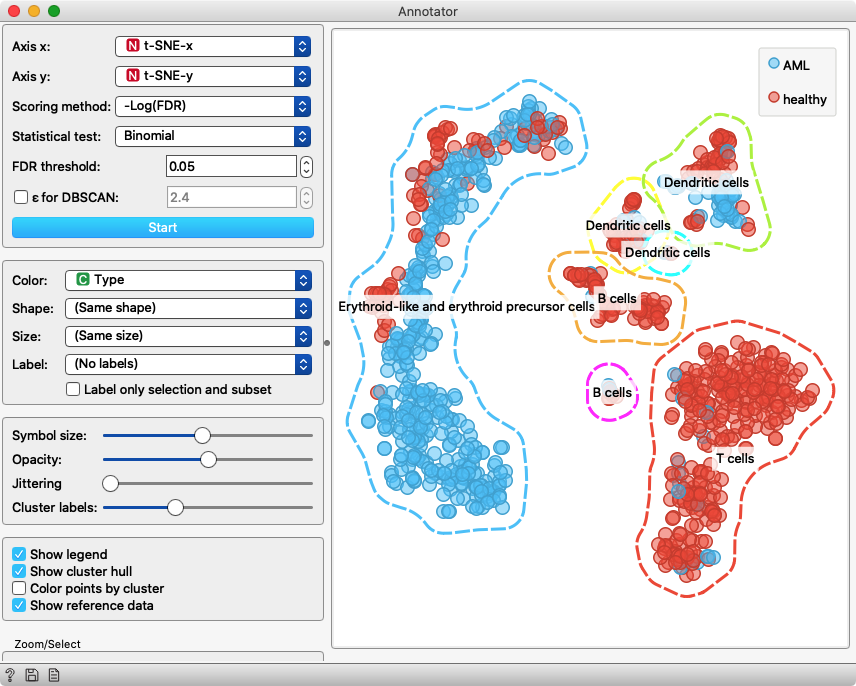
\includegraphics[width=0.6\textwidth]{annotation}}
\end{figure}

\subsubsection{Research Design and Methods}
\begin{description}
	\item[Overview.] 
The overview of the research in the proposed project is presented in Fig.~\ref{fig:approach}. The figure shows how we will integrate the target gene expression data and data on clinical trials with additional knowledge bases and other available data sets. It also exposes the key scientific approaches we will address to find:
\begin{enumerate}
\item which, on their own, are the key molecular markers for survival,
\item which are the combinations of molecular entities that can jointly, in aggregation correlate with survival,
\item which are characterizations of markers that can help us in understanding of the process and interpret the results of the analysis.
\end{enumerate}
While all of the above are clearly the issues that could be addressed by molecular biologists, due to sheer volume of data and additional information in available data and knowledge bases they can only be tackled through means of computational analysis and discovery approaches. The principal challenge of the project is how to combine these different sources, and use modern data mining approaches to support knowledge discovery to provide interpretable and operational hypotheses to biomedical researchers and drug developers. In the description below, we first enlist the data sources on which we will apply our marker discover process, then enlist a set of computational approaches which we will develop and use, and comment on their implementation within an existing visual programming-based data mining framework.

\begin{figure}
\floatbox[{\capbeside\thisfloatsetup{capbesideposition={right,top},
capbesidewidth=0.4\textwidth}}]{figure}[\FBwidth]
{\caption{\small\bold{Knowledge-based analysis to biomarker discovery.} We aim to combine our target data set with transcription and survival data from clinical trials with other available data sets and knowledge bases to gain in speed, accuracy and interpretation of results. Substantial part of our project deals with exploratory data interfaces, which combine visualization of data, identified biomarkers and models. Together, computational approaches for biomarker discovery and visualization approaches for making these findings explicit and placing them in the context of entire search space (e.g., {\em marker maps}) will assist us in explainable, semi-automatic discovery process. The methods we will, in every step shown in the figure, emphasize the role of domain expert and assist, rather than provide black-box decisions.}
\label{fig:approach}}
{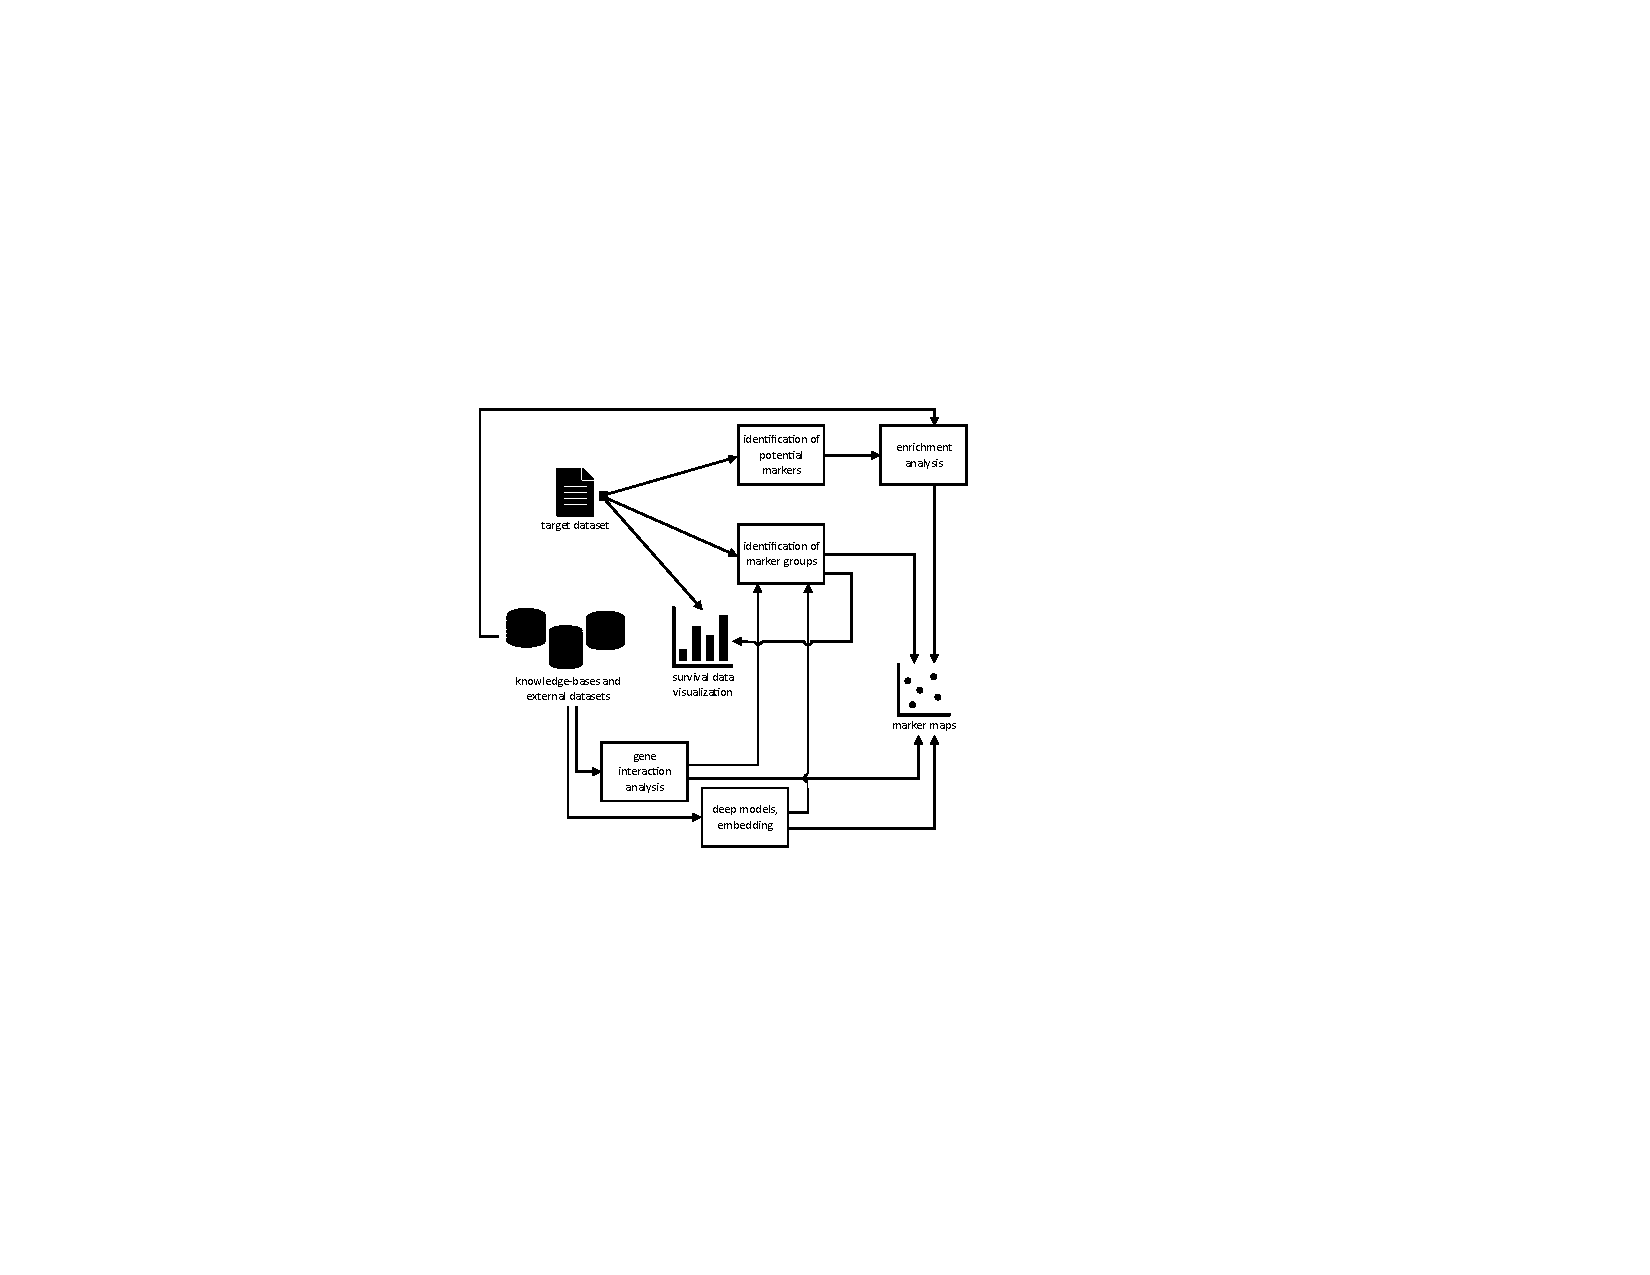
\includegraphics[width=0.6\textwidth]{approach}}
\end{figure}


% \begin{figure}
% 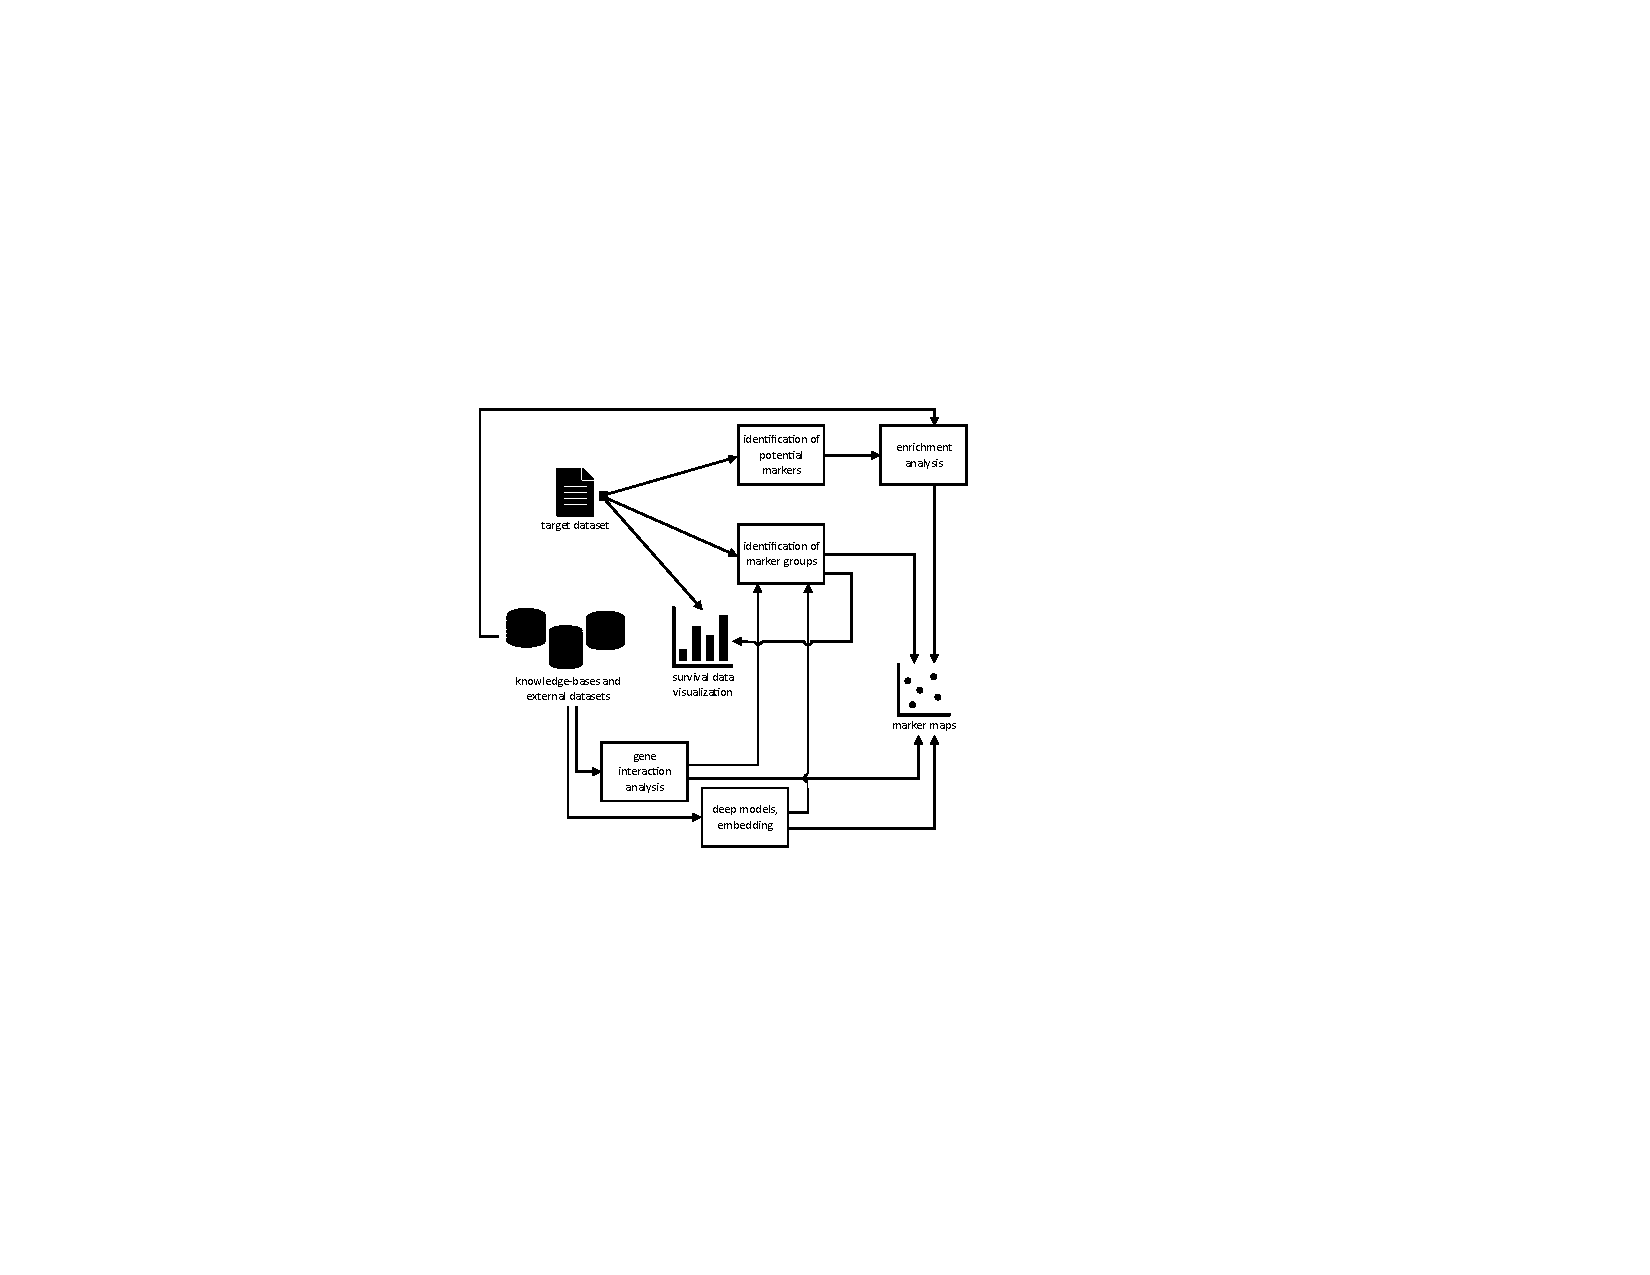
\includegraphics[width=0.48\textwidth]{approach}
% \caption{An example of a Kaplan-Meier plot for two gene expression-dependent conditions associated with patient survival. In panel a), the survival function is substantially higher for a group of patients with highly expressed microRNA hsa-mir-149. The difference is not so evident in the panel b) and microRNA hsa-mir-496. We could say that hsa-mir-149 is hence a better biomarker for survival. In biomarker discovery, one of the tasks is to rank genes and RNA molecules according to the degree of separation between corresponding survival signatures when a gene is expressed and not expressed.}
% \label{fig:approach}
% \end{figure}


	\item[Material and Data Sets.] Four types of data sets will be gathered, organized and used in the project:
	\begin{description}
		\item[DS1] Transcription data from The Cancer Genome Atlas database\myurl{https://www.cancer.gov/tcga}~\cite{24071849} and Gene Expression Omnibus\myurl{https://www.ncbi.nlm.nih.gov/geo/}~\cite{23193258}.
		\item[DS2] Survival analysis data from clinical trials from The Cancer Genome Atlas database.
		\item[DS3] Transcription and clinical trial data managed by Genialis.
		\item[DS4] Simulated data sets.
	\end{description}
	The data from DS1 and DS2 are fragmented; datasets have to be integrated, so that the clinical trial data is aligned with a corresponding transcription data. Methodological reports on development of computational techniques, including those we have cited in the related work, would refer to data repositories but would seldom publish the reorganized data ready to be used in off-the-shelf software packages. Our project aims to break with this practice and compile a data repository with aligned clinical and transcription data sets ready for benchmarking and comparing biomarker discovery techniques.
	
	Genialis d.o.o. already has a collection of such align datasets which comes from their existing partnerships with some major pharmaceutical companies. The data is private, but will be shared with us in the project for testing and validation purposes.

	We will also construct a set of simulated datasets, where variables representing biomarkers will be placed by design. The datasets will serve for testing and benchmarking of the proposed methods.

	The project will additionally use other sources of information, which, for the reasons of convenience, will be queried for information specific for the project and will internally be represented as additional data sets. These include, but are not limited to:

	\begin{description}
		\item[DS6] Gene function annotations from Gene Ontology (GO) consortium.\myurl{https://www.geneontology.org}.
		\item[DS7] Various pathways from KEGG, Kyoto Encyclopedia of Genes and Genomes.\myurl{http://www.geneontology.org}.
		\item[DS8] NDEx pathway data base.\myurl{http://www.ndexbio.org/}
		\item[DS9] Various marker gene data bases, including CellMarker\myurl{30289549} and PanglaoDB
		\myurl{https://panglaodb.se}~\cite{30951143}.
	\end{description}

	\item[Computational Approaches, Data Mining and Bioinformatics.] Computational approaches and development of data mining methods will include:
	\begin{description}
		\item[Data organization (task T1).] The project will develop a computational platform with access to the common, server-based databases that will store transcriptome and survival data from third parties and participating SME Genialis. We will use standard software engineering practices to construct this architecture (file data server with secure HTTP access, HTTP- based queries, components on clients to access the data). We will locally store the data from other information sources like gene ontologies and pathways to allow for fast computation and utility of such information, and for these reuse existing server and database architecture of Orange~\cite{XXX}. Overall, the software engineering task here is to hide all the details of data access and query from the user to allow access to these functions with a single click and focus on data analysis and interpretation.
		\item[Gene ranking (T2.1).] We will use standard log-rank test to compare two or more survival curves and hence estimate a selection of gene and its expression threshold to break observed cases to subpopulation. Log-rank test will be used as a baseline. We will compare the inferred ranking of genes to modeling approaches, where we will infer survival models first, and then estimate the information value of its constituents (genes) either directly for linear models (e.g. Cox proportional hazards models) or indirectly. Advanced models will include random survival forests~\cite{22088987} and deep learning~\cite{29482517,29634719}. Indirect measurements of informatively will include game theoretic approaches such as SHAP\myurl{https://github.com/slundberg/shap}~\cite{32607472}.
		\item[Gene set enrichment analysis (part of T2.1)]. We will use gene set enrichment analysis~\cite{1239896,} to interpret the results of biomarker ranking and to inspect what are the commonalities in terms of functions and pathways of the best-ranked genes.
		\item[Feature construction and gene set identification (task T2.2).] We will direct and indirect feature selection techniques. With direct technique we will select a set of genes (potential markers) and observe their predictive performance with any of the survival modeling techniques. The quality of the set will be estimated through predictive performance of the model. An alternative approach will use model-based feature selection, like $\ell 1$ regularization of Cox and network models.
		\item[Gene interaction analysis (T2.3)] will examine possible combination of genes in their combined effect to the survival function. We plan to use model-based evaluation of gene pairs (T2.1) and represent results in interaction maps (T2.6) and networks.
		\item[Knowledge-infused biomarker discovery (T2.4)] will limit the search for useful combination of features in task T2.2 to genes with common functional or pathway labels, that is, preferably to those that already associated with investigated pathology in the literature. The success of this approach will be measured through gains in algorithm speed and reduction of search space to be considered, while requesting identification of the gene sets of similar quality to those from exhaustive search.
		\item[Deep learning (T2.5)] will employ variational autoencoders~\cite{} for embedding to represent marker candidates with latent vectors, that is, position them in the latent space where we can easily examine their relatedness and the structure of marker space. We will construct autoencoders from gathered collection of transcription data and clinical data sets (task T1), and then use transfer learning~\cite{} to adapt the model to specific target dataset. The embedded representations of potential markers will provide ground to construct interpretable visualisations of the search space (e.g., task T2.6).
		\item[Gene interactions maps (T2.6)] will render information from tasks T2.3 and T2.7 and provide means for graphical explanation and presentation of search space, exploratory data analysis, and visual interpretation. To render gene maps we will use our own variant of t-SNE~\cite{vanDerMaaten2008} called openTSNE\myurl{https://github.com/pavlin-policar/openTSNE}~\cite{policar2019}, which can preserve global structure.
		\item[Annotation of point-based visualizations] will equip gene maps (task T2.6) and other point-based visualizations of gene and marker search space with functional and pathway labels. We will use this approach to provide assisted interpretation of the search space, and assist the domain experts in relating top markers to explanation of their relatedness and biological annotation. In development of this technique we will extend the approach that we have previously developed for single-cell gene expression analysis (see Fig.~\ref{XXX}).
	\end{description}

	\item[Software Implementation.] Over the past two decades, we have been developing a comprehensive data analysis suite called Orange\myurl{https://orangedatamining.com}~\cite{}. Orange has been used by thousands of users and is a toolbox of choice in training of data science in hundreds of universities\myurl{https://orangedatamining.com/blog/2021/2021-01-11-orange-in-classroom/}. Orange features a scripting and a visual programming environment. Visual programming offers an intuitive means of combining known analysis and visualization methods into powerful applications. Orange includes a set of visual components for functional genomics (Fig.~\ref{XXX}) that enable users who are not programmers to manage transcription data flow and to customize their analysis by combining common data analysis tools to fit their needs~\cite{}. Orange framework will be used to implement methods proposed in this project and offer them to the community within an open-source model.

	Within the project, we will develop a set of components that will be specific to the problem in our project, but also general enough to be used in other survival analysis tasks. The new set of components we foresee to develop are those for survival modeling, accuracy estimation, biomarker ranking, identification of groups of markers, gene embedding, and construction of survival-based gene interaction maps. Orange includes components that are also crucial to the proposed project, but that have already been developed or have been at least prototypes. These include the access to some of the gene annotation libraries, components for gene set enrichment, GO browser, and a set of visualization tools including t-SNE and Kaplan-Meier curves.

	\item[Experimental Validation.] We will use the data sets DS1 to DS4 to experimentally validate the both the computational techniques and the visual interfaces we will construct in the project. There are three aspects of validation we would like to assess:
	\begin{itemize} 
		\item \bold{predictive performance}, where we will compare the list of inferred biomarkers to those published in the literature, and compare the results of our marker discovery techniques to those already published;
		\item \bold{interpretability}, which will be assessed with domain experts working with Genialis, a participating SME. The assessment of interpretability will be both quantitative, in terms of how well can we link the list of identified biomarkers to the known functional and pathway labels, and subjective, in terms of agreement of domain experts with proposed result;
		\item \bold{usability}, where we will use hands-on workshops with domain experts to assess if they can use the developed tool independently after three-hour training.
	\end{itemize}
\end{description}

\subsection{Available research equipment over 5.000 €}

The project will use the computational infrastructure of Bioinformatics Laboratory of University of Ljubljana, which includes CPU cluster (about 500 processors), NFS storage (about 500 TB), and a cluster of GPU processors (about 20 GPUs), collectively valued at about 200.000 EUR. We will require no special computational equipment besides the existing for the proposed project.

\subsection{Project management}

The project will join two highly compatible R\&D teams. The Bioinformatics Laboratory from University of Ljubljana will bring to the project its extensive expertise in data mining, machine learning, bioinformatics, and computational phenotyping. The project will be co-financed by Genialis, a data science and drug discovery company focused on new ways to treat disease. Blending computational biology and AI-based methods, Genialis merges and models data at the intersection of clinical and translational medicine. Genialis is trusted by biopharma and big pharma alike, to validate targets, predict biomarkers and optimally position novel drugs. Together, Genialis and its partners are bringing improved solutions to drug discovery to change people's lives.

The project will be managed by UL (project manager). The management of the project will be organized through regular meetings of the management board, with one appointed representative from each institution, and through regular meetings of the project members. The collaboration platform will be based on GitHub and will be made available in the earliest stage of the project.

We will complete the project in three years. Fig.~\ref{fig:timeline} gives the detailed time line of the projects.


% Detailed implementation plan and timetable
% gantt
% risks and remedies

\subsection*{References}

\patchcmd{\thebibliography}{\section*{\refname}}{}{}{}

\begin{multicols}{2}
\footnotesize
\setlength{\parskip}{0em}
\renewcommand{\baselinestretch}{1.0}
\bibliographystyle{abbrv345}
\bibliography{main}
\end{multicols}

\end{document}
